\def\difficulty{2}
\sujet{Morphological Attribute Filtering}\index{Mathematical Morphology!Attribute Filters}
\begin{note}This tutorial aims to test the attribute morphological filters for gray-level images. The objective of such filters is to remove the connected components of the level sets which do not satisfy a specific criterion (area, elongation, convexity...).\end{note}
%
%\noindent The different processes will be applied on the following synthetic images:

%

\noindent Fig.\ref{fig:morphological_attribute_filtering:enonce:examples} are presented some results of attribute filtering applied on the grayscale image.

\vspace*{-5pt}

\begin{figure}[H]
\centering\caption{Attribute filtering examples.}%
\subfloat[Binary image.]{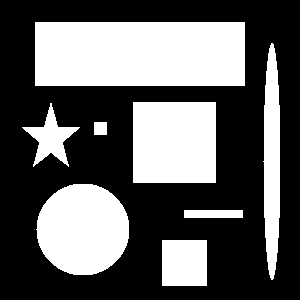
\includegraphics[width=.3\linewidth]{toy.binary.png}}\hfill
\subfloat[Grayscale image.]{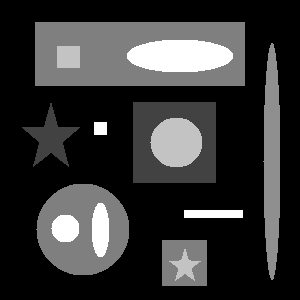
\includegraphics[width=.3\linewidth]{toy.png}}\hfill
\subfloat[Filtering by area.]{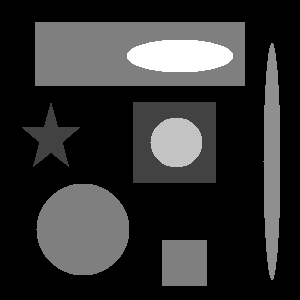
\includegraphics[width=.3\linewidth]{toy.areaOpening.png}}

\vspace*{-5pt}

\subfloat[Filtering by elongation.]{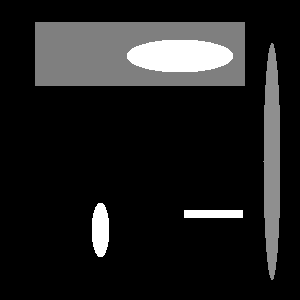
\includegraphics[width=.3\linewidth]{toy.elongThinning.png}}\hfill
\subfloat[Filtering by con\-ve\-xi\-ty.]{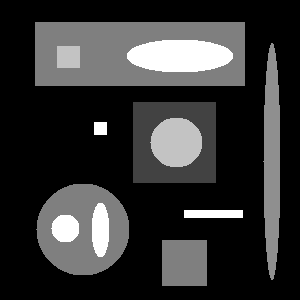
\includegraphics[width=.3\linewidth]{toy.convThinning.png}}\hfill
\subfloat[Filtering objects larger than a square.]{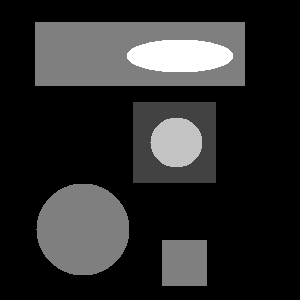
\includegraphics[width=.3\linewidth]{toy.recOpening.png}}%
\label{fig:morphological_attribute_filtering:enonce:examples}%
\vspace*{-8pt}%
\end{figure}
%%

\vspace*{-5pt}

\noindent A {\it binary connected opening} $\Gamma_x$ transforms a binary image $f$ given a pixel $x$, by keeping the connected component that contains $x$ and removing all the others.\\
{\it Binary trivial opening} $\Gamma_T$ operates on a given connected component $X$ according to an increasing criterion $T$ applied to the connected component. If the criterion is satisfied, the connected component is preserved, otherwise it is removed according to:\vspace*{-2pt}
\begin{eqnarray}
\Gamma_T(X)=\left\{
\begin{array}{cc}
X & \text{if } T(X)=\text{true}\\
\emptyset & \text{if } T(X)=\text{false}
\end{array}
\right.
\end{eqnarray}
In general, one or more features of the connected component, on which the filter is applied, are compared to a given threshold defined by the rule.\\
{\it Binary attribute opening} $\Gamma^T$, given an increasing criterion $T$, is defined as a binary trivial opening applied on all the connected components of $F$. This can be formally represented as:\vspace*{-8pt}
\begin{eqnarray}
\Gamma^T(F)=\bigcup_{x\in F}\Gamma_T(\Gamma_x(F))
\end{eqnarray}

If the criterion $T$ evaluated in the transformation is not increasing, e.g., when the computed attribute is not dependent itself on the scale of the regions (e.g. shape factor, orientation, etc.), the transformation also becomes not increasing. Even if the increasingness property is not fulfilled, the filter remains idempotent and anti-extensive. For this reason, the transformation based on a non-increasing criterion is not an opening, but a thinning. In this case, one speak about a {\it binary attribute thinning}.

Attribute openings and thinnings introduced for the binary case can be extended to grayscale images employing the threshold decomposition principle. A grayscale image can be represented by thresholding the original image at each of its graylevels. Then, the binary attribute opening can be applied to each binary image and the {\it grayscale attribute opening} is given by the maximum of the results of the filtering for each pixel and can be mathematically represented as:\vspace*{-3pt}
\begin{eqnarray}
\gamma^T(f)(x)=\max\{k; x\in \Gamma^T(Th_k(f))\}
\end{eqnarray}
\vspace*{-3pt}\vspace*{-\baselineskip}

\noindent where $Th_k(f)$ is the binary image obtained by thresholding $f$ at graylevel $k$.

The extension to grayscale of the binary attribute thinning is not straightforward and not unique. For example, a possible definition of a {\it grayscale attribute thinning} can be analogously defined as Equation (3). However, other definitions are possible, according to the filtering rule considered in the analysis (max, min, subtractive, direct...). Again, if the criterion $T$ is increasing (i.e. the transformation is an opening), all the strategies lead to the same result.

Attribute openings are a family of operators that also includes openings by reconstruction. If we consider a binary image with a connected component $X$ and the increasing criterion "the size of the largest square enclosed by $X$ must be greater than $\lambda$", the result of the attribute opening is the same as applying an opening by reconstruction with a squared structuring element of size $\lambda$.

\vspace*{-8pt}
\section{Binary attribute opening/thinning}
\vspace*{-6pt}
We are going to implement and test some binary attribute filters according to different criteria (area, elongation, convexity).
\begin{qbox}
\begin{itemize}
	\item Regarding the area criterion, implement the associated binary attribute opening. Test on the binary image.
	\item Regarding the elongation criterion, implement the associated binary attribute thinning (non-increasing criterion). Test on the binary image. 
\end{itemize}
\end{qbox}

\vspace*{-6pt}

\begin{mcomment}
\begin{mremark}
 Use the function \texttt{bwpropfilt}.
\end{mremark}
\end{mcomment}

\begin{pcomment}
\begin{premark}
 Code your own function \pinline{bwFilter} based on \pinline{regionprops} from \pinline{skimage.measure}.
\end{premark}
\end{pcomment}



\section{Grayscale attribute opening/thinning}\vspace*{-6pt}
We are going to extend the binary filters to grayscale images.
\begin{qbox}
\begin{itemize}
	\item Implement the decomposition operator into binary sections.
	\item Conversely, implement the reconstruction operator from binary sections.
	\item Implement and test the grayscale attribute filters according to the following criteria: area, elongation, convexity.
\end{itemize}
\end{qbox}

